% tBPSguide.tex v2.1 released November 2014

\documentclass{tBPS2e}

\usepackage{epstopdf}% To incorporate .eps illustrations using PDFLaTeX, etc.
\usepackage{subfigure}% Support for small, `sub' figures and tables
\usepackage{lmodern}
\usepackage{color}
\usepackage[utf8]{inputenc}
\usepackage{float}
\usepackage{lineno}
\usepackage{tikz}
\RequirePackage{fix-cm}


\theoremstyle{plain}
\newtheorem{theorem}{Theorem}[section]
\newtheorem{lemma}[theorem]{Lemma}
\newtheorem{corollary}[theorem]{Corollary}
\newtheorem{proposition}[theorem]{Proposition}

\theoremstyle{definition}
\newtheorem{definition}{Definition}

\theoremstyle{remark}
\newtheorem{remark}{Remark}
\newcommand{\noteCM}[1]{\footnote{\textcolor{red}{#1}}}
\newcommand{\noteJK}[1]{\footnote{\textcolor{blue}{#1}}}
\newcommand{\noteDT}[1]{\footnote{\textcolor{green}{#1}}}

\begin{document}

%\jvol{00} \jnum{00} \jyear{2014} \jmonth{November}

\articletype{Research Article}

\title{\textit{Urban and building multiscale co-simulation: case study implementations on two university campuses}}

\author{Clayton Miller\textsuperscript{a}%
$^{\ast}$\thanks{$^\ast$Corresponding author. Email: miller.clayton@arch.ethz.ch}, 
Daren Thomas\textsuperscript{a},
J\'er\^ome K\"ampf\textsuperscript{b},
and Arno Schlueter\textsuperscript{a}\\
\vspace{6pt}
\textsuperscript{a}{\em Architecture and Building Systems (A/S), Institute of Technology in Architecture (ITA), ETH Z\"urich, Z\"urich, Switzerland};\\
\textsuperscript{b}{\em Solar Energy and Building Physics Laboratory (LESO-PB), Ecole Polytechnique F\'ed\'erale de Lausanne (EPFL), Lausanne, Switzerland}
\received{Submission for review on April 30, 2016} %TARGETED!
}

\maketitle

\begin{abstract}
    This paper describes the co-simulation process of the building and urban
    scale models of two campuses of higher education buildings in Switzerland.
    The campuses are modeled at both the building level, using the EnergyPlus
    simulation engine, and at the urban scale using the CitySim engine. A co-
    simulation framework is used to execute simulations from both engines
    concurrently with an exchange of information to leverage the various
    strengths of each. In the first case study, on-site weather and measured
    performance data are then compared to the output from two modeling
    scenarios: building-scale simulation using EnergyPlus and co-simulation of
    the engines. A partial calibration process is implemented to reconcile the
    simulations with the measured data of a targeted office building on
    campus. In the second case study, the co-simulation results are compared
    to the both the CitySim simulation engine. The results
    show that coupling of EnergyPlus with CitySim resulted in a -15.5\% and
    -7.5\% impact on cooling consumption and a +6.5\% and +4.8\% impact on
    heating consumption as compared to solo simulations of each of the engines. Challenges encountered with the urban scale
    calibration and the strengths and weaknesses of the developed process are
    discussed.
\end{abstract}

\begin{keywords}
Building-scale simulation, Calibrated energy models, CitySim, Co-simulation, EnergyPlus, Urban-scale simulation 
\end{keywords}


% {\abstractfont\centerline{\bfseries Index to information contained in this guide}\vspace{12pt}
% \hbox to \textwidth{\hsize\textwidth\vbox{\hsize19pc
% \hspace*{-12pt} {1.}    Introduction\\
% \hspace*{7pt} {1.1.}  The \textit{tBPS} document class\\
% \hspace*{7pt} {1.2.}  Submission of \LaTeX\ articles\\
% \hspace*{24pt}        to the journal\\
% {2.}    Using the \textit{tBPS} class file\\
% {3.}    Additional features\\
% \hspace*{10pt}{3.1.}  Title, authors' names, abstract \\
% \hspace*{24pt}        and keywords\\
% \hspace*{10pt}{3.2.}  Additional footnotes to the title \\
% \hspace*{24pt}        or authors' names\\
% \hspace*{10pt}{3.3.}  Lists\\
% {4.}    Some guidelines for using standard\\
% \hspace*{6pt}         features\\
% \hspace*{10pt}{4.1.}   Sections\\
% \hspace*{10pt}{4.2.}   Illustrations (figures)\\
% \hspace*{10pt}{4.3.}   Tables\\
% \hspace*{10pt}{4.4.}   Landscape pages\\
% \hspace*{10pt}{4.5.}   Theorem-like environments\\
% \noindent \hspace*{7pt} {4.6.}   Typesetting mathematics\\
% \hspace*{24pt} {4.6.1.}   Displayed mathematics\\
% \hspace*{24pt} {4.6.2.}   Bold math italic symbols\\
% \hspace*{24pt} {4.6.3.}   Bold Greek\\
% \hspace*{24pt} {4.6.4.}   Upright Greek characters  \\
% \hspace*{50pt}            and the upright partial \\
% \hspace*{50pt}            derivative sign  \\}
% \hspace{-24pt}\vbox{\noindent\hsize19pc
% \hspace*{7pt} {4.7.}   Acknowledgements \\
% \hspace*{7pt} {4.8.}   Funding \\
% \hspace*{7pt} {4.9.}   Notes \\
% \hspace*{7pt} {4.10.}   Supplemental material \\
% \hspace*{7pt} {4.11.}   References \\
% \hspace*{24pt} {4.11.1.}  References cited in the \\
% \hspace*{54pt}            text \\
% \hspace*{24pt} {4.11.2.}   The list of references\\
% \hspace*{7pt} {4.12.}   Appendices \\
% {5.}    Example of a section heading \\*
% \hspace*{7pt}   including \textsc{small caps}, \textit{italic}, \\*
% \hspace*{7pt}   and bold Greek such as ${\bm\kappa}$ \\
% {6.}   {\em tBPS} journal style \\
% \hspace*{10pt}{6.1.}   Hyphens, en rules, em rules \\ \hspace*{27pt}and minus signs\\
% \hspace*{10pt}{6.2.}   References \\
% \hspace*{10pt}{6.3.}   Maths fonts\\
% \noindent   {7.}   Troubleshooting\\
% {8.}   Fixes for coding problems\\
% {9.}   Obtaining the tBPS2e class file\\
% \hspace*{10pt}{9.1}  Via the Taylor \& Francis \\
% \hspace*{24pt}       website \\
% \hspace*{10pt}{9.2}  Via e-mail\\ }}}

\linenumbers

\section{Introduction}
\noteCM{Clayton's notes are red!}\noteJK{Jerome's notes are blue!}\noteDT{Daren's notes are green!}

Urban scale building performance simulation is a process that empowers the
analysis and optimization of cities. Urban populations are growing around the
world at an unprecedented rate. A transition from urban to rural is underway and
2.5 billion people are expected to join cities throughout the world by the year 2030
\citep{UnitedNations:2014vn}. Expansions of entire districts and even cities
is not an uncommon phenomenon, especially in East Asia and Africa. Urban scale
modeling is in the midst of an intense focus on the research community with
six key areas of practice: technology design, building design, urban climate,
systems design, policy assessment, and land use and transportation
\citep{Keirstead:2012ct}. The ability to simulate the interaction between
large collections of buildings enables the development and testing of
optimization and planning scenarios for this new development
\citep{Dorer:2013vt}.

The CitySim simulation engine is an example of such a program designed and
optimized for urban-scale simulation. CitySim is an urban performance
simulation engine that comprises a solver module as well as a graphical user
interface. It focuses on the energy flows of multiple simplified building
models and their interdependent relationship with their urban climate
\citep{Robinson:2009tm}. CitySim includes building thermal, urban radiation,
occupant behavior, and plant/equipment models integrated as a single
simulation engine. CitySim simulates multiple buildings up to city scale using
simplified models to achieve a good compromise between modeling
accuracy, computational overheads, and data availability. Each building's
thermal behavior is based on an electrical analogy using a two node resistor-
capacitor network. The internal lighting, people, and miscellaneous loads are
modeled using a simplified occupancy-based approximation. The heating,
ventilation, and air-conditioning (HVAC) systems are modeled using a single
equation that approximates the total mass flow rate required to meet the
sensible and latent loads of each building as a whole. Each of these
simplifying approximations empowers the urban-scale simulation to have
reasonable execution times on the number of buildings being
simulated.

Building performance simulation is a mature domain of research relative to
urban scale efforts. The use of whole building simulation engines originated
in the 1960s with the US government's development of the BLAST and DOE-2
hourly energy simulation programs \citep{Lawrie:2001vf}. In 1996, development
on a new simulation engine, EnergyPlus, began in order to combine the
advantages of previous efforts in a single, modular program. EnergyPlus, as a
result, has become a popular choice in detailed whole-building performance
simulation due to the breadth of mechanical, renewable, and electrical systems
that can be modeled. EnergyPlus specifically excels in its ability to model
unique mechanical system types such as decoupled centralized cooling
\citep{Miller:2010wa} and low exergy heating and cooling systems
\citep{barbara:2015tz}. Additionally, EnergyPlus is designed to provide a high
resolution in which internal loads and natural ventilation technologies can be
modeled in detail at the building level.

Both building and urban-scale simulation domains have rightfully chosen
boundary conditions that reflect their key goals while seeking to minimize the
input parameters necessary and run-times of the engines themselves. This focus
results in certain deficiencies concerning modeling various phenomena.
For example, urban scale simulation highly simplifies the building systems and
internal load models, thus making a retrofit analysis at the systems level
difficult. And whole building simulation in EnergyPlus neglects many of the
various contextual consideration of the urban environment such as long wave
radiation exchange with adjacent surfaces and localized urban weather effects
\citep{Lawrie:2001vf}.%\noteDT{ref?}

To address the deficiencies of the individual engines, the current
effort seeks to couple building and urban scale simulation. The research in
this paper is part of a larger coupling effort in which various engines are
connected and co-simulated to create a more comprehensive analysis of the
urban scale \citep{Dorer:2013vt,Allegrini:2012kx}. The target is the
computational interface between the building energy model, using EnergyPlus,
and the urban energy model using CitySim. An overview of the larger scope is
shown in Figure \ref{fig:UMEM} and the context of the coupling task appears as 
the interface between the City Energy Simulation (CES) model and the
Building Energy Simulation (BES) model. The scales and models contained in the 
urban environment context include the Urban-Scale Model (UC Model), the UMC model using OpenFoam, 
and the Meteorological Meso-scalce (MM model). On the database side, Revit, global 
information systems (GIS), and building information systems (BIS) are utilized.

% \noteDT{can we do phrasing? prettyplease?}

The coupling and co-simulation process is implemented on two case studies in
Switzerland. The first case study is the ETH Z\"urich Hoenggerberg campus in
Z\"urich, Switzerland. The campus was modeled in the CitySim simulation engine
and co-simulated using work-flow automation. The target of this case study is
to evaluate the differences between the coupled and solo EnergyPlus
simulations based on the variables exchanged. This scenario includes the use
of measured data for heating and cooling within their respective seasons to
compare to the simulation results. The second case study is the EPFL campus in
Lausanne, Switzerland. The objective of this scenario is to evaluate the
differences between coupled and uncoupled versions of the CitySim simulation
engine.

 % with a target on the use of these models for building retrofit analysis.\noteDT{I do not understand the preceding sentence. Neither will the reviewer}

\begin{figure}[H]
\centering
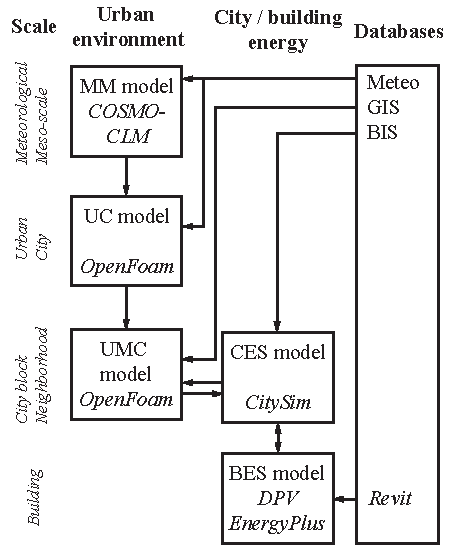
\includegraphics[scale=0.7]{figures/UMEM_overview_new}
\caption{EnergyPlus and CitySim coupling are part of the wider context. Each
block in the diagram represents an environment, with the tool/engine name in
italics (\citep{thomas2014multiscale}, adapted from \citep{Dorer:2013vt})}
\label{fig:UMEM}
\end{figure}

This paper describes the achievement of several objectives:
\begin{enumerate}
  \item Automate of the process of simultaneous meta-data extraction from a
  building information model (BIM) for the creation of both building and
  urban-scale performance models for a real-world campus of buildings
  \item Co-simulate the urban and building scale models through concurrent information exchange
  \item Implement a simplified calibration procedure for the first scenario by 
  reconciling the co-simulation output results for a target building using measured energy
  performance data from the campus energy information system (EIS)
\end{enumerate}

% \noteDT{s/have/has/}

The first two objectives have been demonstrated in a simplified context in
previous literature \citep{thomas2014multiscale,Miller:2015vk}. The innovation
in the current publication is an extension of this research through the
modeling and co-simulation of real-world case studies. With respect to the
third contribution, to the best of the authors' knowledge, no previous study
has compared the results of a building and urban-scale co-simulation procedure
to measured data from a real-world campus.% \noteDT{:)} 

\subsection{Previous multi-scale coupling studies}
Previous attempts of information exchange have been implemented between
simulation engines at various scales. Much of the initial co-simulation work
in the literature is done at the subsystem and building-scale. Previous studies
have analyzed strong and loose coupling of engines at this scale
\citep{Trcka:2010cr,Wetter:2011kh}. Coupling of building-scale simulation with
urban-scale computational fluid dynamics (CFD) is attempted for modeling
natural ventilation \citep{Zhang:2013vx} and to improve energy prediction
\citep{Bouyer:2011eha}. A comprehensive review of energy and airflow modeling
of neighborhoods and university campuses was published that includes
strategic aspects of coupling different %\noteDT{did you mean: "strategic"?}b
types of models \citep{Srebric:2015gq}. EnergyPlus has been coupled with ENVI-
met, a micro-climate computational fluid dynamics (CFD) program
\citep{Yang:2012cr}. It was also coupled with simplified lumped parameter
models to facilitate comparison with measured sensor data
\citep{Martin:2015fj}. While not directly coupled, EnergyPlus and the TEP Urban Canopy Model program were connected
through a modified weather file to quantify the influences of urban localized weather effects
on whole building simulation \citep{Bueno:2011hi} and urban weather generation
\citep{Bueno:2013hh}.
% Recent work in coupling geographic information systems platforms like GIS and simplified performance modeling techniques have also been completed \citep{Fonseca:2015bm}\noteDT{this is not technically a simulation coupling}.
% \subsection{Urban scale performance simulation}

\section{Methodology}\label{Methodology}
% Portions of the following methodology is developed in previous literature and is reiterated to set the context for Section \ref{Implementation}. The previously published research is clearly outlined at the beginning of each subsection.

\subsection{Coupling process} 
The coupling process of a simplified single zone
model and contextual surrounding buildings is described in previous studies
\citep{thomas2014multiscale}, which forms the basis for the methodology
in the current effort. This process utilizes the Design Performance Viewer
(DPV) and associated workflow. The DPV is a tool written to extract and
simulate an EnergyPlus input data file (IDF) from an
Autodesk\textsuperscript{TM} Revit\textsuperscript{TM} BIM
\citep{Schlueter2009}. The central philosophy behind the tool is a rapid simulation
of the building information model from the earliest design possible that can be
used throughout the life-cycle of the building including retrofit analysis
\citep{Miller:2014tu}. This process is achieved by augmenting the information
in the BIM with default values and abstracting information not relevant for
energy simulation. The tool already has a simplified notion of surrounding
buildings, which are modeled in the BIM as simple mass objects without further
information and are exported as shading surfaces to EnergyPlus. This
functionality is used for creating the CitySim mass scene and leads to a crude
model of the urban context of the building. The current DPV philosophy of
allowing the designer to iterate rapidly on early design decisions based on
feedback about the performance of the design remains. This approach includes
streamlining the process where running a simulation requires no effort from
the designer due to automatic creation of input files, execution, and analysis
of the results.% \noteDT{not sure the second reference includes coupling...}

The coupling process of EnergyPlus and CitySim is shown in Figure
\ref{fig:OverallWorkflowProcess}. The solid lines depict the co-simulation of EnergyPlus
and CitySim and the dotted lines depict solo simulations of either EnergyPlus or CitySim. 
First, the DPV is used to extract an
EnergyPlus simulation model from the BIM. The DPV utilizes the Revit API to
extract geometrical information about the building and the physical properties
of walls, windows, doors, roofs, and floors. This information is encoded in the
BIM model as wall types, roof types, floor types as well as window and door
families. Wherever possible, the tool uses the layering and materials of the
construction types, enhancing them with physical attributes relevant to
EnergyPlus. Where not defined, it assumes default values.

\begin{figure}[H]
\centering
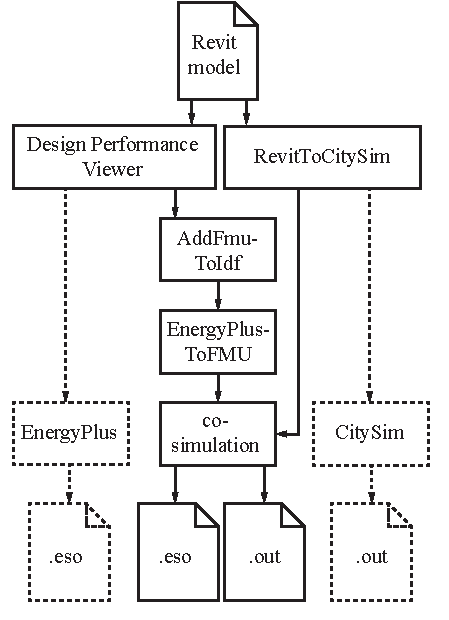
\includegraphics[scale=0.7]{figures/UMEM_Workflow}
\caption{Overview diagram of the coupling process including tools and outputs \citep{thomas2014multiscale}}
\label{fig:OverallWorkflowProcess}
\end{figure}

Next, geometry is created to be used in both the CitySim and EnergyPlus models
as buildings and surfaces surrounding the building targeted in the IDF. This
feature of the DPV is used for including shading surfaces in the EnergyPlus
simulation model: it uses so-called \emph{mass objects} in the BIM model as
surrounding buildings. The DPV model views these buildings as a series of
shading surfaces. A transformation is added to the DPV model that produces an
input file for the CitySim solver. This file uses an XML format describing the
buildings in a scene for simulation, including their construction types,
geometry, and systems for heating and cooling. The main BIM is extracted to the
CitySim scene as one of the buildings to be simulated, with the properties of
the construction types matching those in the DPV model. The glazing ratio is
calculated based on the window and wall areas of the DPV model. Shading
surfaces are grouped into buildings based on the mass object from which they were extracted. These neighboring buildings use default construction properties for walls and roofs, and we assign them a default glazing ratio.
These defaults can be overridden by custom properties applied to the mass
objects in the BIM much in the same way as the model elements of the main
building are enriched with DPV information.

As of version 8.1.0, EnergyPlus supports exporting a simulation model as a
Functional Mock-up Unit (FMU) \citep{Nouidui:2014hq,Anonymous:ZZTfF80-}. This
feature introduces new IDF objects to specify the interface such an FMU
exposes. These objects define which output variables are exported by the FMU
and which variables are imported. The FMU export functionality is closely
linked to the Energy Management System (EMS) of EnergyPlus. Co-simulation
exchange variables either mimic an EnergyPlus schedule, an EMS variable or
drive an EMS actuator. Since the model used by CitySim to simulate a building
is more abstract than the model used by EnergyPlus, the EMS is used to
aggregate certain values. CitySim does not model windows separately. Therefore,
a weighted average of window and wall surface temperatures is calculated with
EMS subroutines.
% \noteDT{@JK: is this last statement correct?}

% It was determined that to export an output variable using the FMU export functionality, the variable itself must also be output with an IDF object of type \emph{Output:Variable} or \emph{EnergyManagementSystem:OutputVariable} in the IDF file as well.

% The process of augmenting the IDF file is automated with the EMS subroutines and FMU export objects. The script \emph{addfmutoidf.py}, written in the Python programming language, uses the \emph{parseidf} module to read in the IDF file and add the new IDF objects based on those found in the model.  This script reads in the list of surfaces defined in the IDF file and produces EMS scripts to aggregate and output the surface temperatures of the wall and the windows as well as any other output objects necessary.

The FMU creation process is the basis for coupling the two models at each
timestep in the simulation. Figure \ref{fig:FMUOverview} illustrates this
process from both the EnergyPlus and CitySim perspective. The augmented IDF
file is fed to the \emph{EnergyPlusToFMI} script \citep{Nouidui:2014bo}. Once
configured, this script produces an FMU file based on the augmented IDF file
and the weather file to be used as well as a DLL file implementing the
Functional Mock-up Interface that can load the IDF file, locate EnergyPlus and
run the simulation.

\begin{figure}[H]
\centering
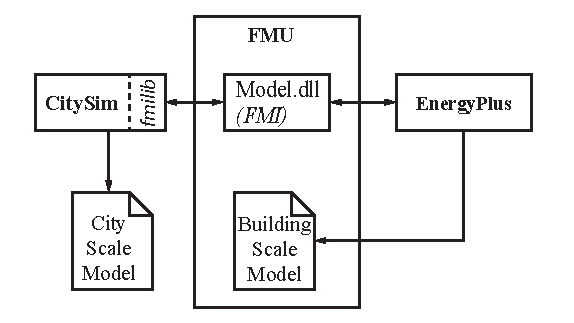
\includegraphics[scale=0.7]{figures/UMEM_FMU_Overview}
\caption{Simulation information exchange between CitySim and EnergyPlus using FMI \citep{thomas2014multiscale}}
\label{fig:FMUOverview}
\end{figure}

% Table \ref{FMUimports} and \ref{FMUexports} outline the variables exchanged between EnergyPlus and CitySim through the FMI. 

% We used the \emph{fmilib} library from the JModelica project to test the FMU produced \citep{Anonymous:ZZTfF80-}. We altered one of the sample programs (\emph{fmi\_import\_cs\_test.c}) to load the FMU, run it and print out the values exported from EnergyPlus. This code was then used as a guide to extending the CitySim solver to load FMUs for co-simulation.

\subsection{Coupled variables}

% On an hourly basis, CitySim performs a heating and cooling needs prediction step. The temperature determination step for the main building is replaced with the results of the EnergyPlus timestep as obtained through FMI library. The FMI library is used to send climatic and occupational data from CitySim to EnergyPlus, and to receive data from EnergyPlus that are further used within CitySim for the next time steps. 
Several key urban-scale weather variables are sent to EnergyPlus from CitySim
to account better for the localized effects of surrounding buildings,
geography and climate conditions. These variables are outlined in Table \ref{FMUimports}. 
They include various outdoor air
conditions such as dry bulb and wet bulb temperatures, dew-point, humidity, wind
speed and direction, and direct and diffuse solar radiation. These variables
overwrite the input weather variables that EnergyPlus obtains from its weather
file input. CitySim is designed to account for physical phenomenon inherent to
urban environments that are often neglected in building-scale simulation
environments \citep{Robinson:2004cr,Robinson:2009tm}. Long wave radiation
exchange between the simulated building and its surroundings is sent to
EnergyPlus; this process is described in detail in Section \ref{lwradiation}.
Finally, CitySim shares its calculated occupancy schedules as it uses a more
robust model of occupants behavior
\citep{Haldi:2011dr}.

% \noteDT{s/climactic/climatic/}
% \noteDT{this sentence, man. i can't even}

\begin{table}[H]
\tbl{Values sent to EnergyPlus from CitySim by the FMU}
{\begin{tabular}[l]{@{}lcc}\toprule
  \bf{Object} &  \bf{Variable Name} & \bf{Description} \\
\colrule
  Outdoor & Outdoor Drybulb & The outdoor dry-bulb temperature in $^{\circ}\mathrm{C}$ \\
 & Outdoor Dewpoint & The outdoor dewpoint temperature in $^{\circ}\mathrm{C}$ \\
 & Outdoor Relative Humidity & The outdoor relative humidity expressed in percent. \\
 & Diffuse Solar & Diffuse horizontal irradiance in W/m$^2$ \\
 & Direct Solar & Beam normal irradiance in W/m$^2$ \\
 & Wind Speed & The outdoor wind speed in m/s \\
 & Wind Direction & The wind direction in degrees\\&&  (N=0, E=90, S=180, W=270) \\
 \hline
 Long Wave Radiation & Environmental Radiant Temp. & Calculated $T_{env}$ from the sky,\\&& ground, and surrounding surfaces \\
 & Environmental Radiant Heat  & Calculated $h_{env}$ from the sky,\\
 & Gain Coefficient & ground, and surrounding surfaces \\
 
 \hline
Zone & Occupation & Fraction of the maximum occupation\\&& (0.0-1.0) overrides the EnergyPlus occupation schedule\\&&  with the CitySim stochastic schedule. \\
\botrule
\end{tabular}}
\label{FMUimports}
\end{table}

Variables sent to CitySim by EnergyPlus at each time step include several
variables related to the calculation of heating and cooling loads of a
targeted building. Table \ref{FMUexports} outlines this list of exchanged variables.
These variables are transferred due to the ability of
EnergyPlus to model more detailed building systems, schedules, ventilation and
internal load types than CitySim. For example, EnergyPlus is flexible enough
to model a detailed radiant heating and cooling system that would be
impossible in CiytSim \citep{barbara:2015tz}. EnergyPlus is an engine
optimized to accurately model building-scale systems. Thus, CitySim can take 
advantage of these models through coupling and co-simulation. EnergyPlus sends
the heating and cooling loads, the surface temperatures of the exterior
surfaces and the ventilation flow rates to CitySim.

%\noteDT{I'm not sure this is proper English. Or American for that
%matter...}

%\noteDT{in table 2: "Values SENT to CitySim..."}
\begin{table}[H]
\tbl{Values sent to CitySim from EnergyPlus by the FMU}
{\begin{tabular}[l]{@{}lcc}\toprule
  \bf{Object} &  \bf{Variable Name} & \bf{Description} \\
\colrule
Wall, Roof & Outside Surface Temperature & The temperature on the outside of the surface in $^{\circ}\mathrm{C}$ \\    
    \hline
Wall & Average Outside Surface Temperature & The (weighted) average temperature of \\
& & the surface on the outside in $^{\circ}\mathrm{C}$. \\
    \hline
Zone & Total Heating Energy & The heating energy in Joules used in this timestep. \\
& Total Cooling Energy & The cooling energy in Joules used in this timestep. \\
& Zone Mean Air Temperature & The mean air temperature in the zone in $^{\circ}\mathrm{C}$ \\
& Ventilation Volume Flow Rate & The flow rate in $\mathrm{m}^3/\mathrm{s}$ (standard density) \\
\botrule
\end{tabular}}
\label{FMUexports}
\end{table}

\subsection{Long wave radiation exchange}
\label{lwradiation}
Long wave radiation exchange in the urban scale environment is coupled in the
co-simulation process. It requires the development of a set of
approximations to reduce the number of coupled variables between the engines
and to account for differences in the methods by which each engine calculates
this value. A detailed description of Long Wave Radiation (LWR) variable
exchange and approximation is found in a previously published study
\citep{Miller:2015vk} on a simplified theoretical case.

In EnergyPlus, LWR exchange for a surface is calculated through the summation
of radiation gain from the ground, sky, and air as seen in Equation
\ref{EPlus_LWR_Ext} and Figure \ref{combinedLWR}a \citep{doe2010energyplus}.
The radiant heat transfer coefficient for each of these environmental
variables is calculated according to Equation \ref{EPlus_h} with $\sigma$ as
the Stefan-Boltzmann constant and $\epsilon$ as the emissivity. A major
assumption of this approach is that the modeled building's surfaces and those
of adjacent buildings are at a uniform temperature and the LWR radiation
exchange is negligible; a situation that is an oversimplification in an urban
scale domain \citep{Evins:2014cf}.
\begin{equation} \label{EPlus_LWR_Ext} 
Q_{LWR,EnergyPlus} = h_{r,grd}(T_{surf}-T_{grd}) + h_{r,sky}(T_{surf}-T_{sky}) + h_{r,air}(T_{surf}-T_{air})
\end{equation}
\begin{equation} \label{EPlus_h} 
h_{r,variable} = \frac{\epsilon\sigma(T^{4}_{surf}-T^{4}_{variable})}{T_{surf}-T_{variable}}
\end{equation}

In comparison, CitySim calculates LWR exchange by calculating an aggregated
equivalent temperature, $T_{env}$, and radiative heat transfer coefficient,
$h_{r,env}$, from surrounding urban surfaces in addition to ground, sky, and
air \citep{Robinson:2009tm}. The calculation for $T_{env}$ is expressed in
Equation \ref{CitySim_Tenv} with the $F$ values being view factors of the
surrounding environment including adjacent surfaces $i=1..n$. $h_{r,env}$ is
based on a first order Talyor development of the numerator of Equation
\ref{EPlus_h} around $(T_{surf}+T_{variable})/2$ and therefore
$Q_{LWR,CitySim}$ is calculated using Equation \ref{CitySim_LWR_Ext}.

\begin{equation} \label{CitySim_Tenv} 
\sigma T_{env}^4 = \sigma F_{sky}T_{sky}^4 +\sigma F_{grd}T_{grd}^4 + \sum_{i=1}^{n} \epsilon_i \sigma F_{i}T_{i}^4
\end{equation}
\begin{equation} \label{CitySim_LWR_Ext} 
Q_{LWR,CitySim} = h_{r,env}(T_{surf}-T_{env})
\end{equation}

In the coupled simulation, EnergyPlus uses the CitySim supplied equivalent
$h_{r,env}$ and $T_{env}$ to calculate weighted $h_{r,sky}$, $h_{r,grd}$, and
$h_{r,air}$ values using the view factors and the sky-to-air split ratio.
Figure \ref{combinedLWR} illustrates the schematic differences between the
solo and coupled simulations on a theoretical example of a target building
with two adjacent buildings with surfaces available for radiation exchange.

\begin{figure}[H]
  \centering
  \includegraphics[width=1.0\textwidth]{figures/LWRCalc_Combined_V3}
  \caption{Comparison of the LWR components between a) Solo EnergyPlus and b) Coupled CitySim/EnergyPlus configuration \citep{Miller:2015vk}
  \label{combinedLWR}}
\end{figure}

\subsection{Work flow automation}
The coupling, simulation and co-simulation process is completely managed
within a program called VisTrails \citep{Anonymous:Cayf2tu7}. The
implementation of this type of work flow is outlined in previous work focused
on automating DPV using the Kepler platform \citep{Thomas:2012wj}. This
process reduces the effort expended by a designer down to pressing a single
button. This functionality allows an iterative design style informed by
readily available simulation results. An automated work flow ties the
various steps together and maintain the effortless iterative design process.
VisTrails enables the coupling of various work flow subprocesses script
initializations, executions of the engines, and the compilation of the
outputs. This tool empowers the coupling of various executable files and their
connecting scripts in graphical diagrams that enhances reproducibility and
process automation \citep{Freire:2014tt}. The VisTrails work flow diagram for
the first case study in this paper is seen in Figure \ref{VizTrails}.

% INSERT VISTRAILS GRAPHIC HERE\noteCM{Daren -- can you give me a good screenshot of the Vistrails for the HPI building? Pretty please.}\noteDT{sure - check out 36-HPI-cosim.pdf in the figures folder}

\begin{figure}[H]
  \centering
  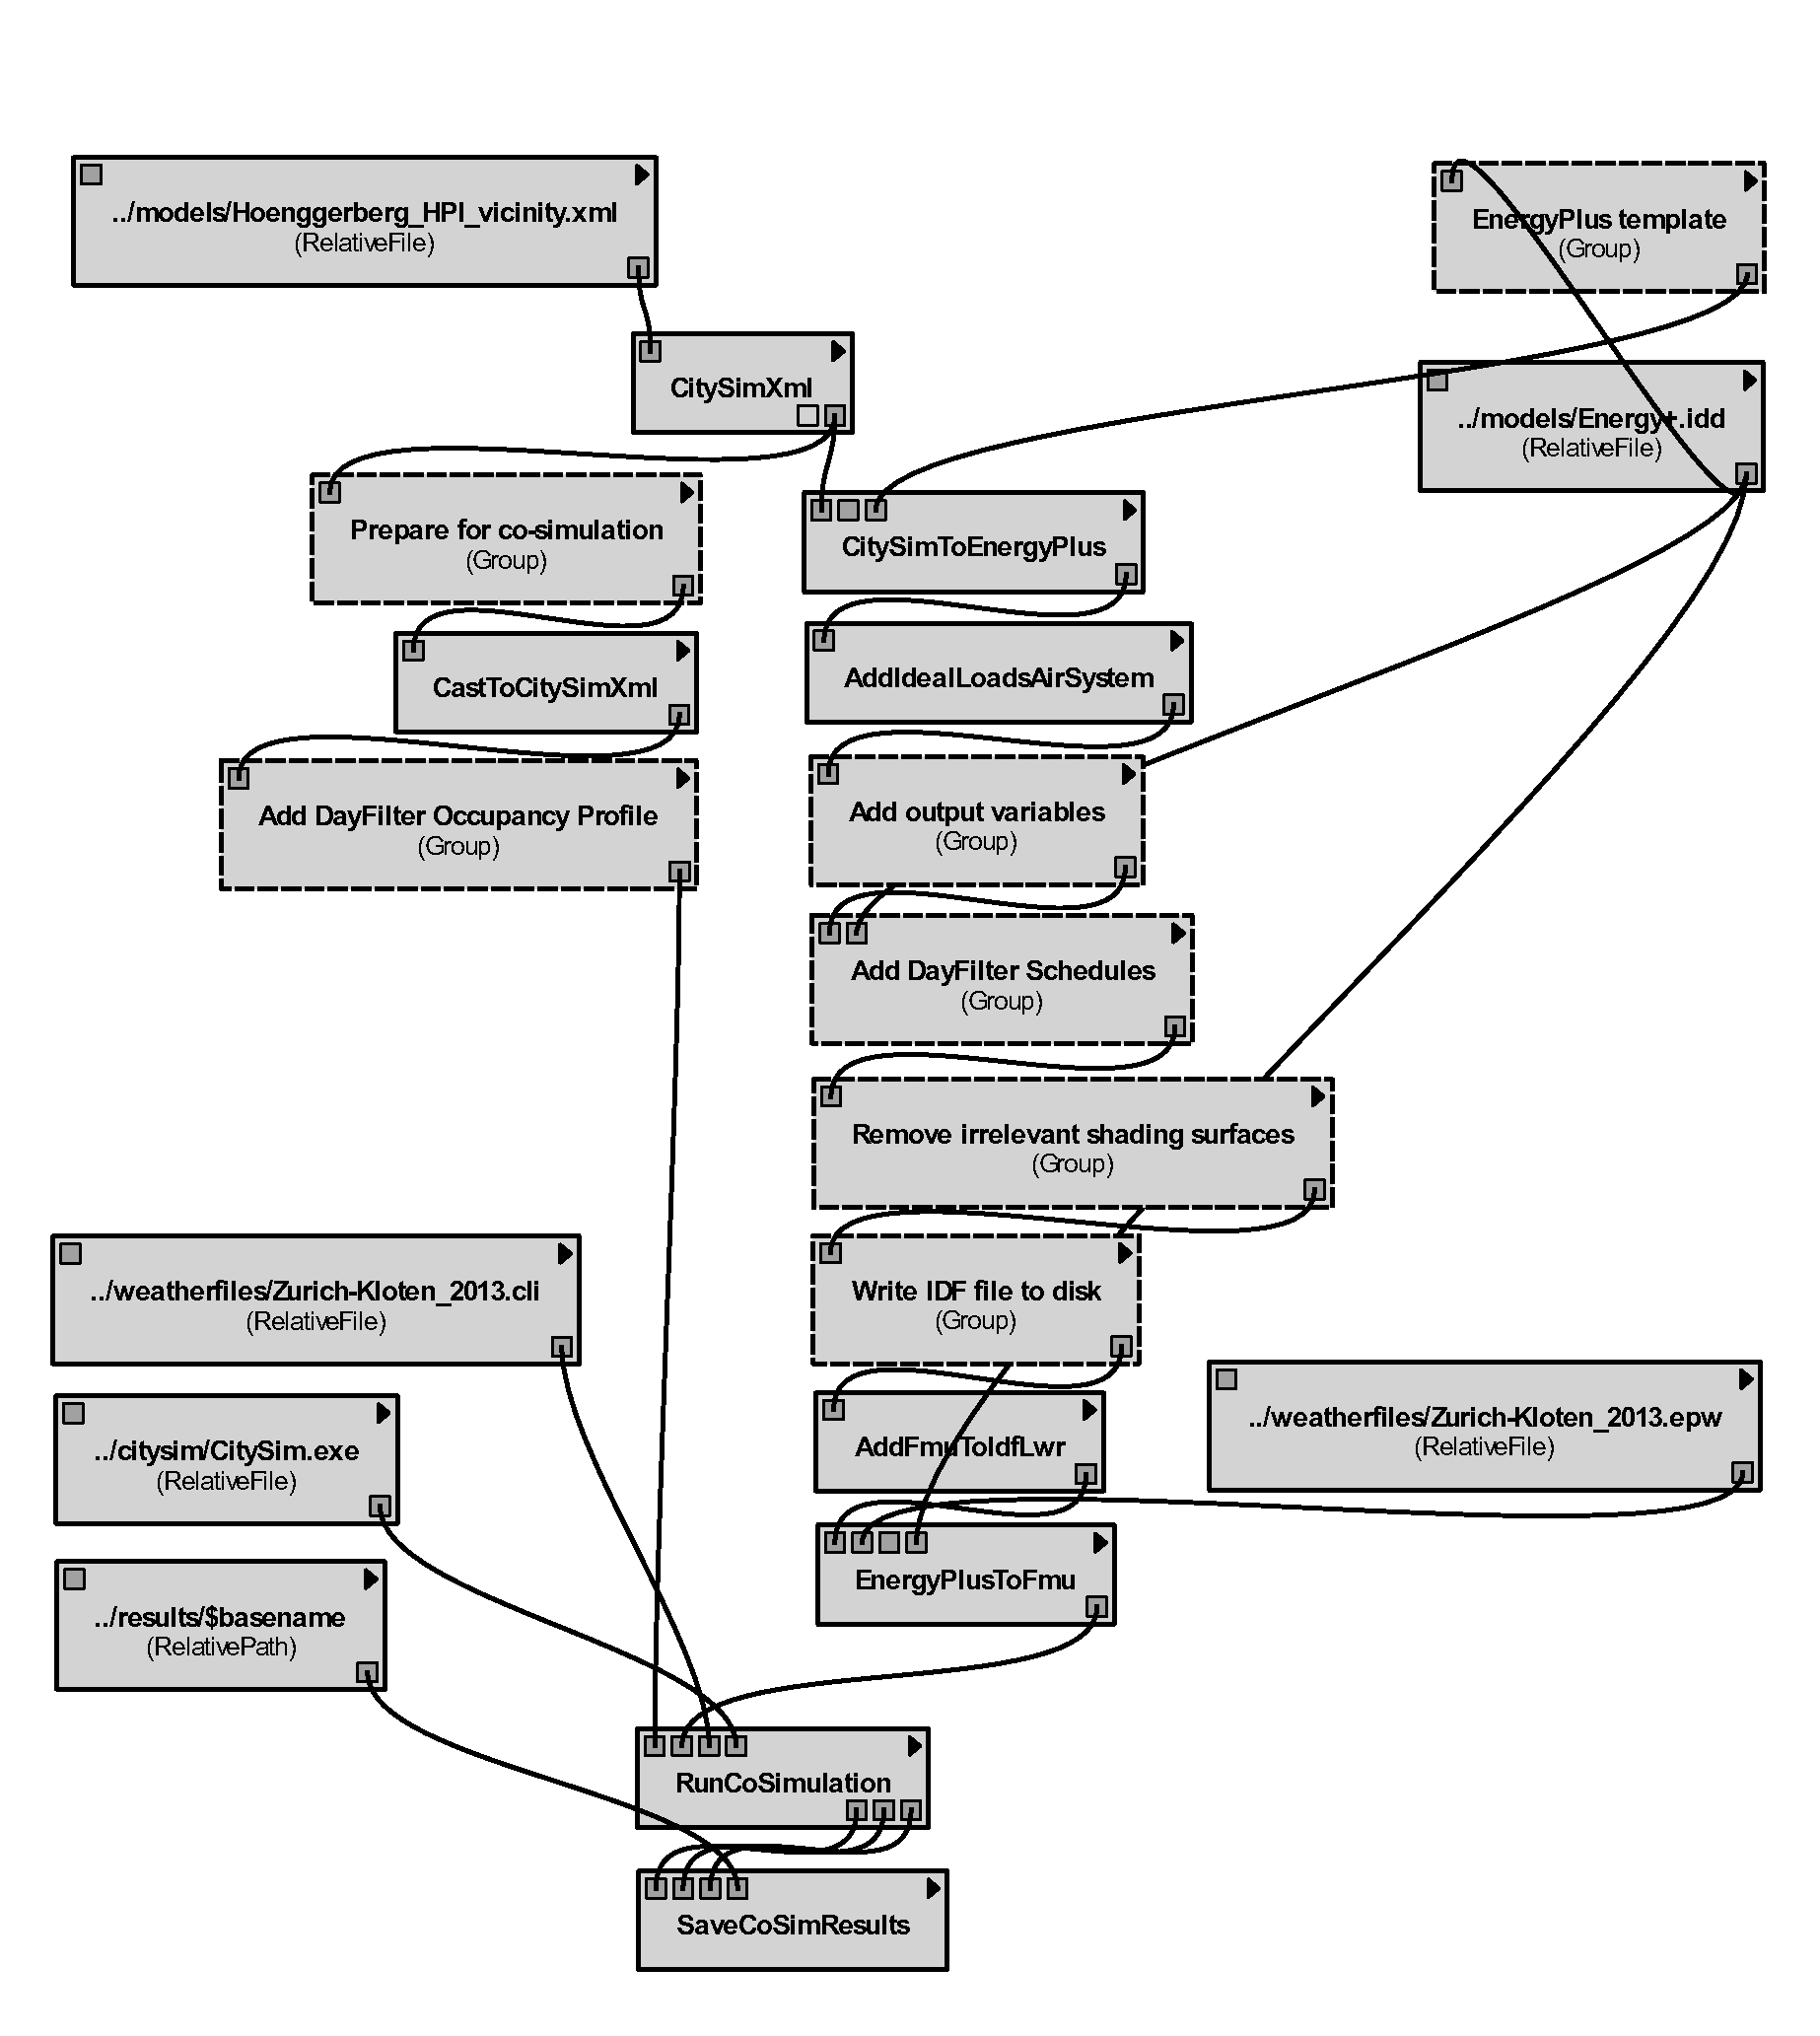
\includegraphics[width=1.0\textwidth]{figures/36-cosim-HPI}
  \caption{Workflow in VizTrails
  \label{VizTrails}}
\end{figure}

\subsection{Simplified calibration}
In the first case study, one aspect of this analysis is the comparison of
actual measured performance of the target building on campus with the
simulation results of the co-simulation. A simplified calibration procedure is
adapted from previous research to compare the measured heating and cooling
data available on campus with various simulation scenarios
\citep{Samuelson:2015jg}. This calibration procedure was utilized in the
performance reconciliation of 18 buildings that were built according to the
LEED Canada protocol and were under review of actualized performance. This
protocol is unique in its analysis process to uncover design model
deficiencies in a step-wise manner, utilizing the most easily accessible
knowledge first and working towards equilibrium between measured and
simulated. There is an appropriate balance between the effort of implementation and value
generated through the calibration process.

% The following steps are the general procedure applied to the targeted buildings:

% \begin{enumerate}
%   \item Using the local weather conditions for the simulation period
%   \item Update simulation based on custom lighting schedules and power densities extracted from the measured data
%   \item Update simulation based on custom plug load schedules and power densities extracted from the measured data
%   \item Account for \emph{unregulated} building loads such as experimental equipment and process loads
% \end{enumerate}
 
\section{Implementation}\label{Implementation and results}
The co-simulation process is implemented on two case studies in Switzerland.
The first is the ETH Z\"urich Hoenggerberg campus in Z\"urich, Switzerland.
The focus of this case study is to quantify the impact of the information
exchange through co-simulation within the EnergyPlus engine. The intent on
this campus was to develop techniques for retrofit analysis using EnergyPlus.
The targeted building on this campus is the HPI Building. Raw measured data is
available for many of the buildings on campus, thus a simplified calibration
procedure is used to reconcile the simulation results.\\

The second case study is the EPFL campus in Lausanne, Switzerland. The
targeted building, in this case, was the Quartier Nord complex. The focus of
this study was to compare the solo and co-simulation output results of CitySim.
Reliable measured data for calibration is not currently available for this
building.

\subsection{Campus case study 1: ETHZ Hoenggerberg Campus}
The ETH Z\"urich Hoenggerberg campus includes 32 higher education facilities
 with spaces allocated to laboratories, office space, lecture halls,
 cafeterias, data centers and other types of similar areas. The campus has a
 centralized energy management system (EMS) that contains 807 energy and water
 measurement points from heating, cooling, electricity, city gas, domestic hot
 water, grey water, and general water consumption. %\noteDT{deleted: "buildings"}

%Figure \ref{fig:pointgraph} illustrates the breakdown of these measurement system data points amongst the campus buildings.

% \begin{figure}
% \centering
% 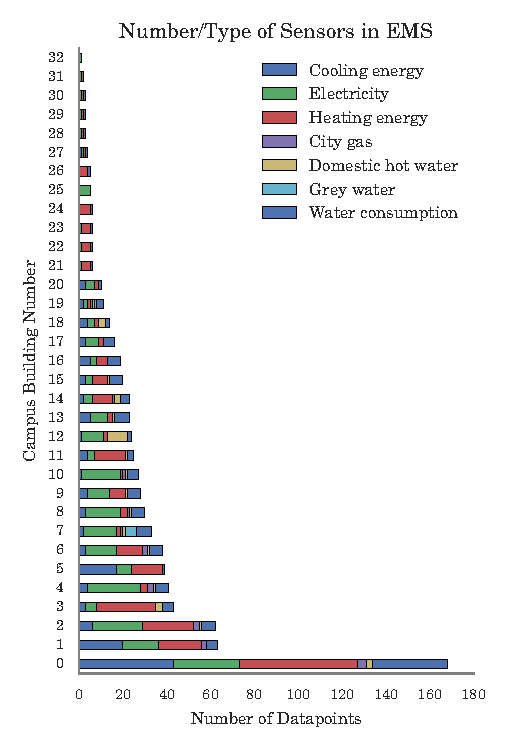
\includegraphics[scale=0.7]{figures/pointbreakdown_anon}
% \caption{Available performance measurement points}
% \label{fig:pointgraph}
% \end{figure}

The focus of the co-simulation process is that the performance of a targeted
building is evaluated through solo and coupled methods. The HPI building on
campus was chosen in this case study due to the amount and quality of measured
data available from the EMS for this building. HPI is a 2,610 square meter
building that is made up mostly of office space and classrooms. It also
includes 400 $m^2$ convenience store and coffee shop. The building is
indicated on a campus map shown in Figure \ref{fig:campusmap} and is shaded
red.

\begin{figure}[H]
\centering
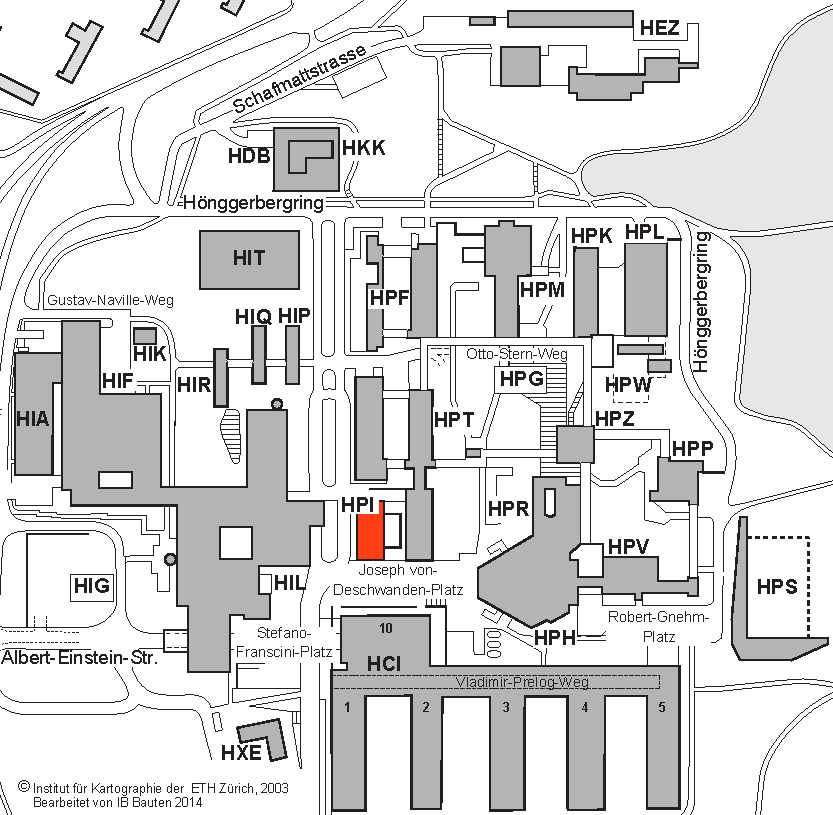
\includegraphics[scale=0.5]{figures/ETH_Hoenngerbergcamp_targetedbuildings_HPI}
\caption{ETH Hoenggerberg campus map with the HPI building shaded red}
\label{fig:campusmap}
\end{figure}

\subsection{Model development}
In order to perform a co-simulation of the targeted buildings, initially a
CitySim model of the campus was developed. Through the workflow automation
process, this geometry was converted into an EnergyPlus input file as seen in
Figure \ref{fig:HPIcampus}. The EnergyPlus input file was then used as an input
to execute EnergyPlus solo and co-simulation processes for the purpose of
simplified calibration, and then to understand the magnitude of difference
between these simulation scenarios.

\begin{figure}[H]
\centering
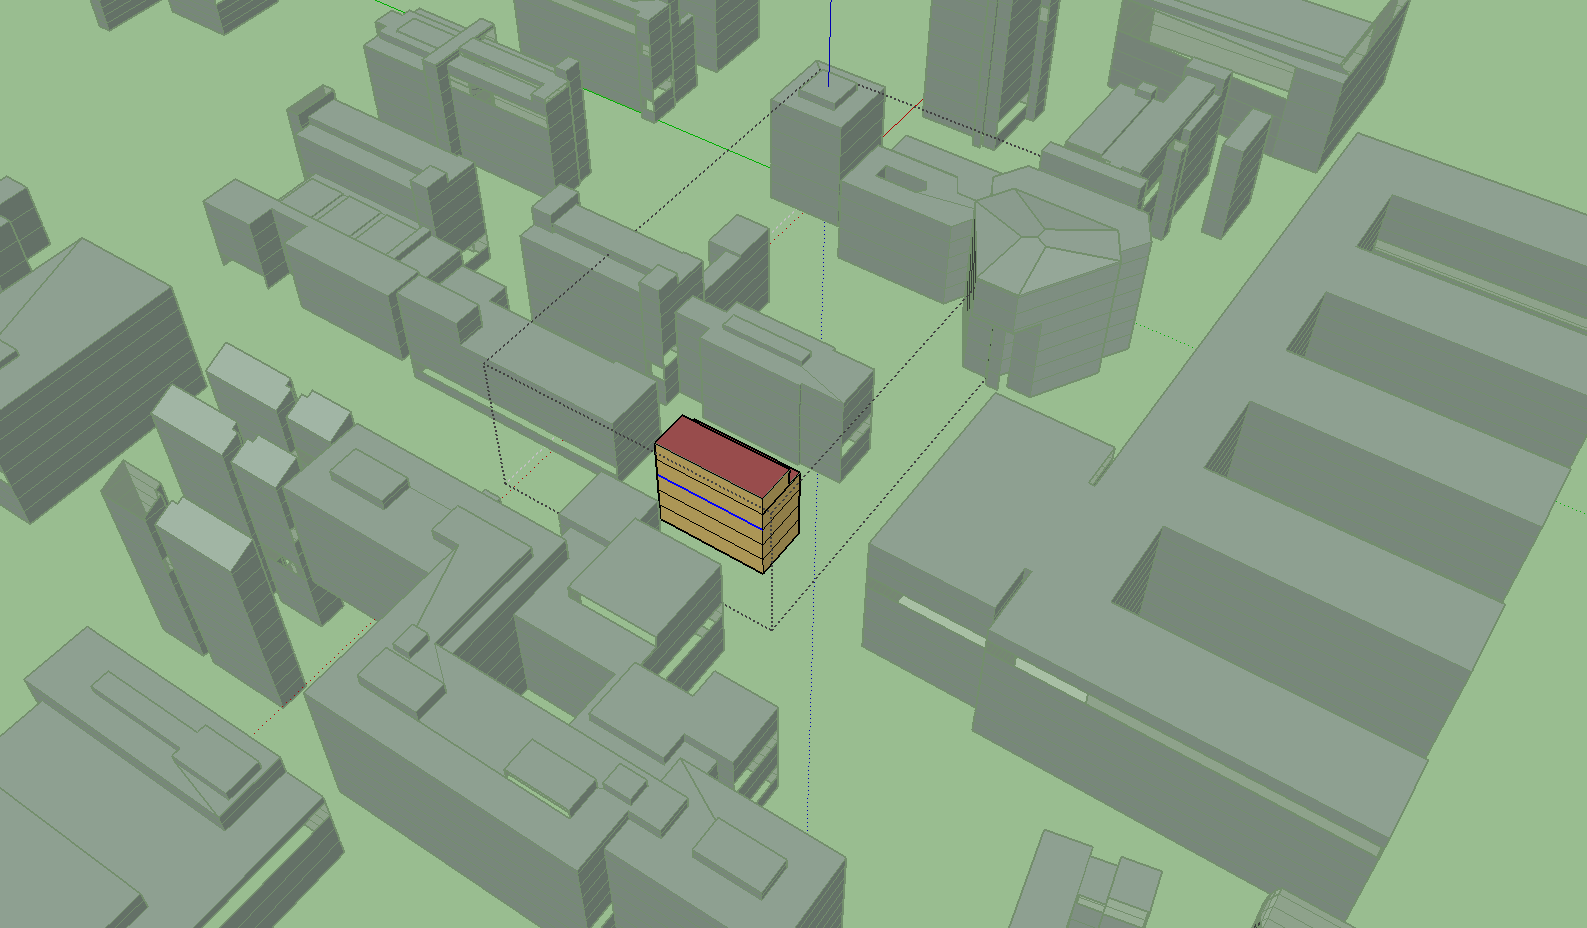
\includegraphics[scale=0.2]{figures/HPI_Campus.png}
\caption{The HPI building EnergyPlus model extracted from the CitySim model. The HPI building is seen
as the light and dark brown building in the center surrounded by gray masses that represent other buildings on 
campus. The graphic is illustrated with OpenStudio for Sketch-up.}
\label{fig:HPIcampus}
\end{figure}

\subsection{Measured data collection and calibration}
Energy data from the HPI building was collected and analyzed in the context of
the simplified calibration procedures. The measured datasets were screened and
aggregated into typical usage profiles to be used for the lighting, plug-
loads, and HVAC equipment availability schedules and power densities. Figure
\ref{fig:hpi_elec_profiles} illustrates the aggregation examples of electrical
energy for the HPI building. This profile was created through a filtering and
clustering process known as \emph{DayFilter} \citep{Miller:2015kr}. Cluster 0 represents
the typical energy profile for Sunday, while Cluster 1 dominates the Saturdays of the data set.
Clusters 2 and 3 make up most of the weekdays of the data set with Cluster 3 being more common in 
non-summer months. These profiles are used to set the availability schedules as inputs into the
EnergyPlus simulation to emulate the way occupants inhabit the building and
how the building management system (BMS) controls the lighting and HVAC
systems. 

\begin{figure}[H]
\centering
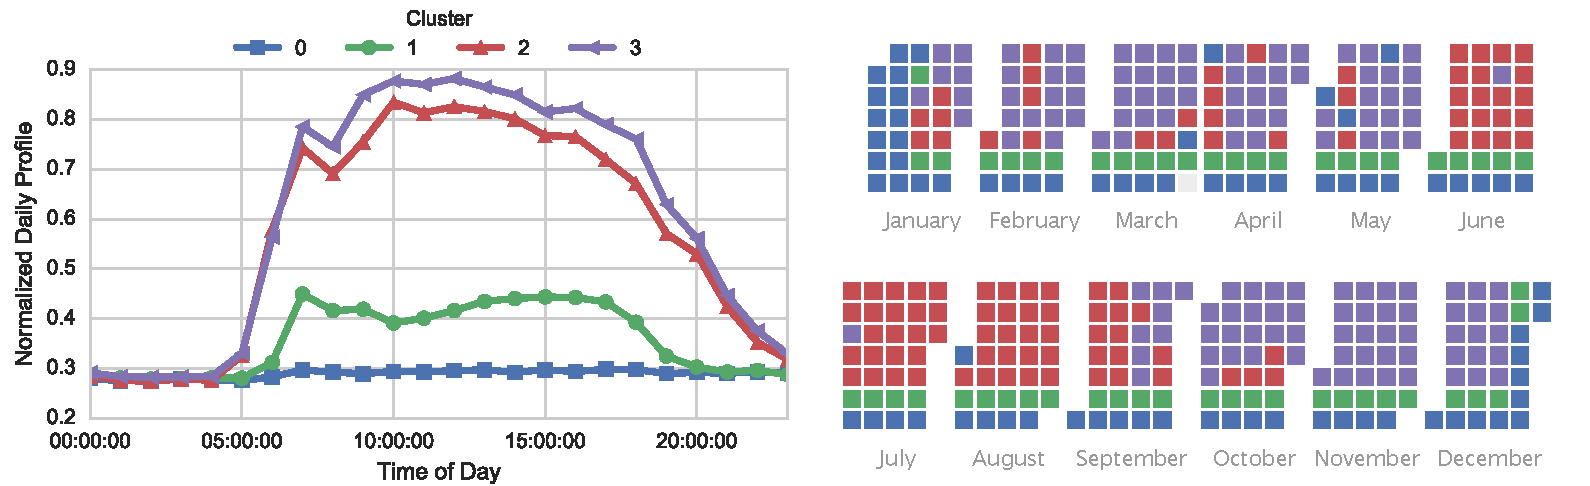
\includegraphics[scale=0.55]{figures/HPI_combinedclusterandcal_5}
\caption{Typical measured data electricity profiles of (left) average daily electrical consumption for each cluster and (right)
color-coded calendar of which days fall within each cluster. The diagram on the right is each month of the year with each row corresponding with
a day of the week (starting with Monday) and each column corresponding to a week of the month.}
\label{fig:hpi_elec_profiles}
\end{figure}

The measured and simulated data from both the co-simulation and EnergyPlus
solo simulation were analyzed in order to understand how both the solo and co-simulations 
compare to real, measured data. The calibration process was undertaken through a series of steps
such as including local weather conditions for the simulation period and
adding custom lighting schedules and power densities extracted from the
measured data. The models were calibrated to the summer season (May-September)
for cooling and the winter season (Jan-April and October to December) for
heating. Figure \ref{fig:hpi_measvssim} illustrates a comparison of the measured data with the
simulations after the tuning process. The final calibrated EnergyPlus solo
model had a normalized mean bias error (NMBE) of -9.36\% and a coefficient of
variation of root mean square error (CVRMSE) of 21.7\% for cooling and -9.36\%
and 29.4\% for heating. These metrics fall within the +/-10\% NMBE and +/-30\%
CVRSME used in this case study for calibration. The
goal of calibration, in this case, is to just bring the models to within a
reasonable range of reality in order to bring more confidence to analysis of
the discrepancies between the solo and co-simulation
scenarios.


\begin{figure}[H]
\centering
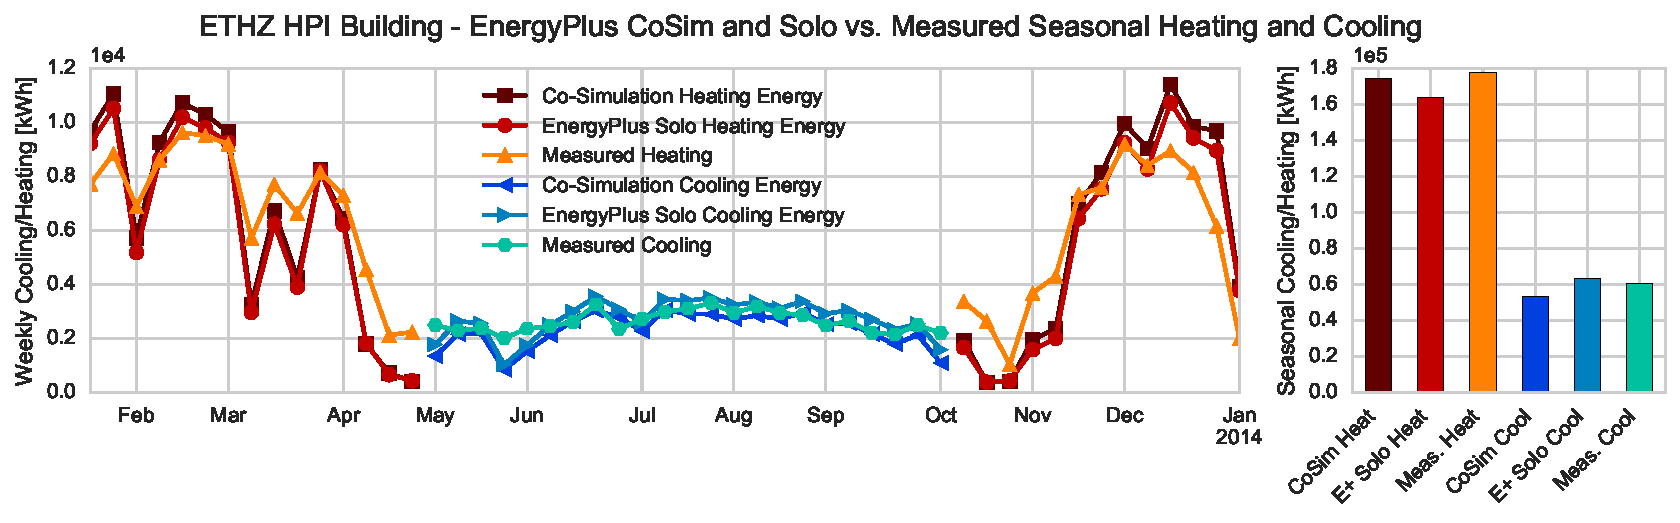
\includegraphics[scale=0.55]{figures/HPI_MeasvsSim}
\caption{HPI Measured vs. Co-Simulation and EnergyPlus Solo for Heating and Cooling Seasons}
\label{fig:hpi_measvssim}
\end{figure}

\subsection{EnergyPlus co-simulation results}
After calibration, a comparison of co-simulation and solo EnergyPlus
simulations is made. For cooling, a discrepancy can be seen between co-
simulation and solo EnergyPlus. Co-simulation decreases the predicted cooling energy by 15.5\%, as seen in Figure
\ref{fig:hpi_energypluscooling}. Figure \ref{fig:hpi_energyplusheating}
illustrates the difference in predicted heating energy consumption across the
test year. A consistent offset exists across the time frame of days in
January, the peak of the heating season. A more varied discrepancy across the
heating months is noticed resulting an overall increase of heating prediction
of 6.5\% due to co-simulation. The exchange of long wave radiation for this
particular site is substantial due to the proximity of surrounding buildings.
These performance differences due to co-simulation are compared to a
theoretical single-zone case study in which there was a 15-30\% increase in
heating energy and a 4-11\% decrease in cooling energy \citep{Miller:2015vk}.
The results from this case study are less extreme on the heating side and more
on the cooling side than the theoretical case study. 

When comparing the solo and co-simulated models to the measured data, it is noticed that 
cooling energy is over-predicted by the solo simulation by 4\%, while co-simulation under-predicted 
by 11.1\%. For heating energy, co-simulation was able to bring the predicted value to within 2\% of 
the measured value for the year, an improvement as compared to the solo simulation, which was 8.5\% less than the measured value.


\begin{figure}[H]
\centering
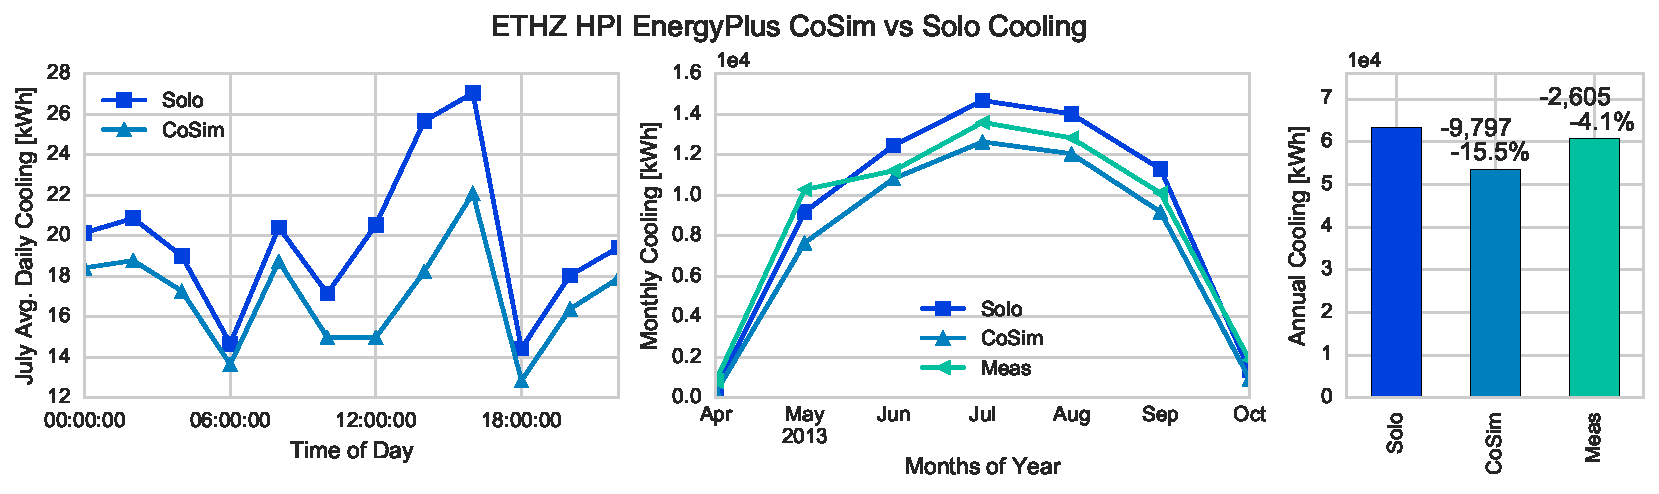
\includegraphics[scale=0.55]{figures/HPI_EnergyPlus_Cooling}
\caption{HPI Co-Simulation vs. EnergyPlus Solo for Cooling}
\label{fig:hpi_energypluscooling}
\end{figure}


\begin{figure}[H]
\centering
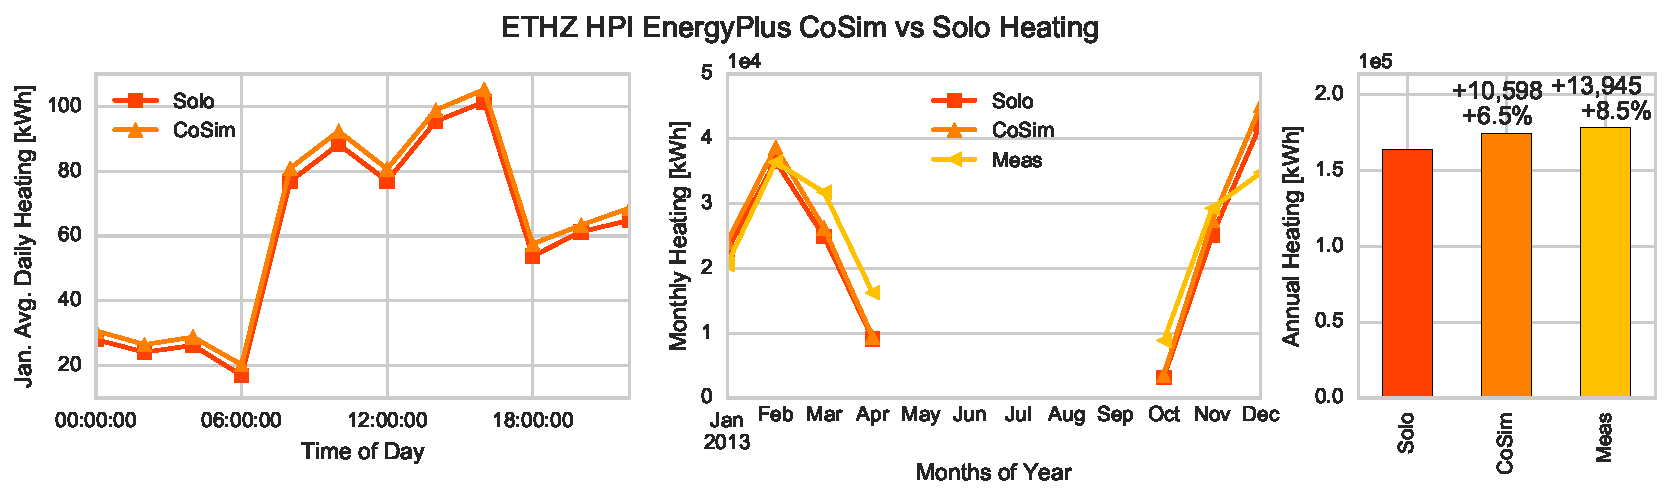
\includegraphics[scale=0.55]{figures/HPI_EnergyPlus_Heating}
\caption{HPI Co-Simulation vs. EnergyPlus Solo for Heating}
\label{fig:hpi_energyplusheating}
\end{figure}


\subsection{Campus case study 2: EPFL Quartier Nord} 
Quartier Nord is a whole new quarter of the École Polytechnique Fédérale de
Lausanne (EPFL) campus located at its northwest corner. This complex includes
a Convention Centre with an auditorium with a maximum capacity of 3000
(seated) people, housing for 516 students, retail and service areas and a
hotel. As a public space, this ensemble is organized around the central plaza as
seen in Figure \ref{fig:quartier_nord_1}). With a particularly strong visual and formal identity, the SwissTech
Convention Centre (STCC) is clearly the key protagonist.  Designed as a
Minergie building, it includes modern energy conversion
technologies to reduce its energy consumption. The focus of the co-simulation
is realized on the STCC, simulated with the nearby buildings for housing,
retail and service areas.

\begin{figure}[H]
\centering
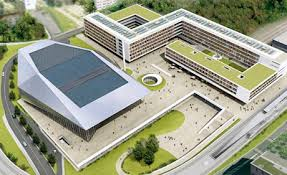
\includegraphics[]{figures/quartier_nord_1}
\caption{The Quartier Nord at EPFL in Lausanne}
\label{fig:quartier_nord_1}
\end{figure}

\subsection{Model development}
The information required in the simulation mainly comprises three parts:
physical, geometrical and operational data. The geometry information including
the shape, dimension, structure and materials was obtained from the Real
Estate and Infrastructure Department of École Polytechnique Fédérale de
Lausanne (EPFL), which was responsible for carrying out the project from call
to tender to construction. However, since the documents provided were full of
details but also conflicting with what has been installed as compared to the
documents before construction, the task to realize a precise model of the
buildings itself is rather tedious. Besides, it is even more challenging to
get the operational data (daily occupancy, lighting, and electrical equipment
usage level and ventilation rate) as the building has only recently been set
in operation mode and as engineers and technicians have been working on
improving the controls. Therefore, due to unreliable monitoring data, the
calibration step of the model was not undertaken.\\

Considering the lack of detailed information about the building, a so-called
detailed reference case was modeled with EnergyPlus \citep{Mauree:2015to} in
which regulation standards applied in the design phase from the SIA norms were
used to complete the missing information. A rendering of this model is seen in
Figure \ref{fig:model_yang}.

\begin{figure}[H]
\centering
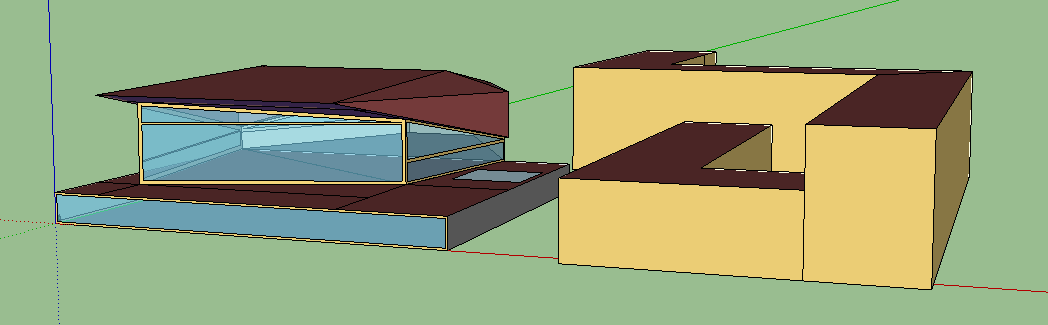
\includegraphics[width=\textwidth]{figures/model_yang}
\caption{The Quartier Nord modeled with OpenStudio for
Sketchup\noteDT{s/sketchup/SketchUp/}. The STCC on the left is the main focus
of the study and is represented by two thermal zones.}
\label{fig:model_yang}
\end{figure}

The corresponding CitySim model was created by exporting a DXF file from
EnergyPlus, and importing it into the Graphical User Interface of CitySim.
Physical characteristics of the building were added to complete the CitySim
model. Finally, the same script as described in Section \ref{Methodology} was
used to export the model from CitySim to EnergyPlus, giving a simplified
EnergyPlus model.\\

\subsection{Comparison of EnergyPlus and CitySim}

Both the CitySim and EnergyPlus engines are utilized in this case study. The
first comparison to observe is the differences between the two engines when
focused on the Quartier Nord building. When simulated in isolation, the
CitySim engine predicts a 28.6\% increase in heating load and a 44.4\%
increase in cooling load as compared to EnergyPlus. This phenomenon is due to
the differences in the way each of these engines calculates heating and
cooling loads. Use of the co-simulation process brings the engines to within
5.4\%. Figure \ref{fig:qn_eplusvscitysim_cooling} illustrates these
differences for cooling and Figure \ref{fig:qn_eplusvscitysim_heating} for
heating.

\begin{figure}[H]
\centering
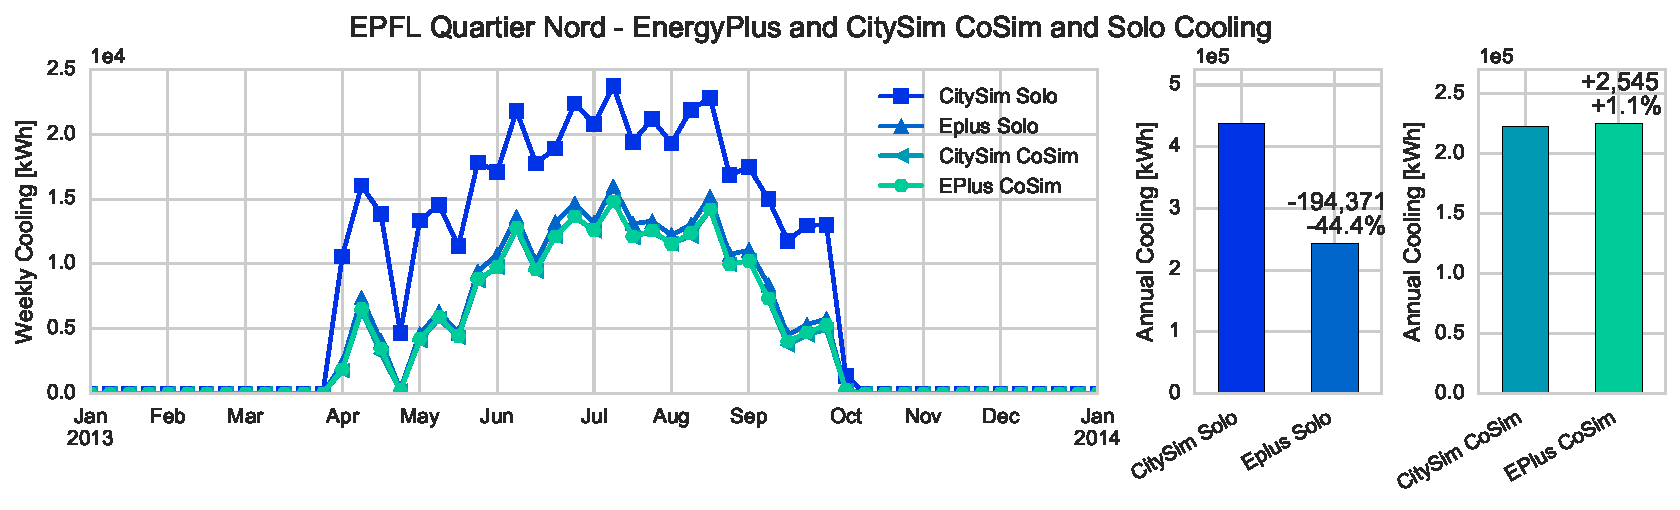
\includegraphics[scale=0.55]{figures/QN_Cooling}
\caption{Quartier Nord CitySim vs. EnergyPlus Solo for Cooling}
\label{fig:qn_eplusvscitysim_cooling}
\end{figure}

\begin{figure}[H]
\centering
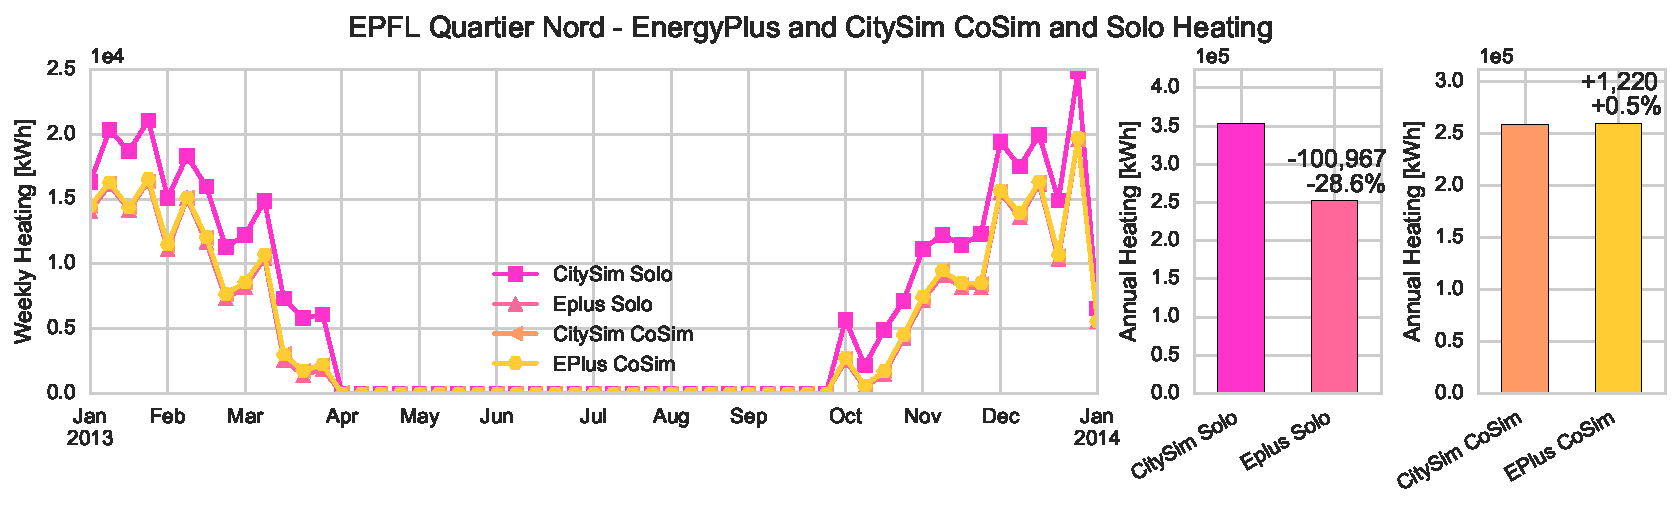
\includegraphics[scale=0.55]{figures/QN_Heating.pdf}
\caption{Quartier Nord CitySim vs. EnergyPlus Solo for Heating}
\label{fig:qn_eplusvscitysim_heating}
\end{figure}


\subsection{EnergyPlus co-simulation results}
The Quartier Nord building is also simulated within the solo and
cosimulation environments. When
focusing on the EnergyPlus results, a 7.5\% decrease in cooling energy is
observed, as seen in Figure
\ref{fig:qn_eplus_cosimvssolo_cooling}. A 2.8\% increase in heating energy is
observed, as seen in Figure
\ref{fig:qn_eplus_cosimvssolo_heating}. These differences are less pronounced
than the HPI and theoretical case studies due to the number and proximity of
surrounding buildings is not as large. Long wave radiation exchange in this situation 
doesn't have as large of an impact on the heating and cooling calculations.


\begin{figure}[H]
\centering
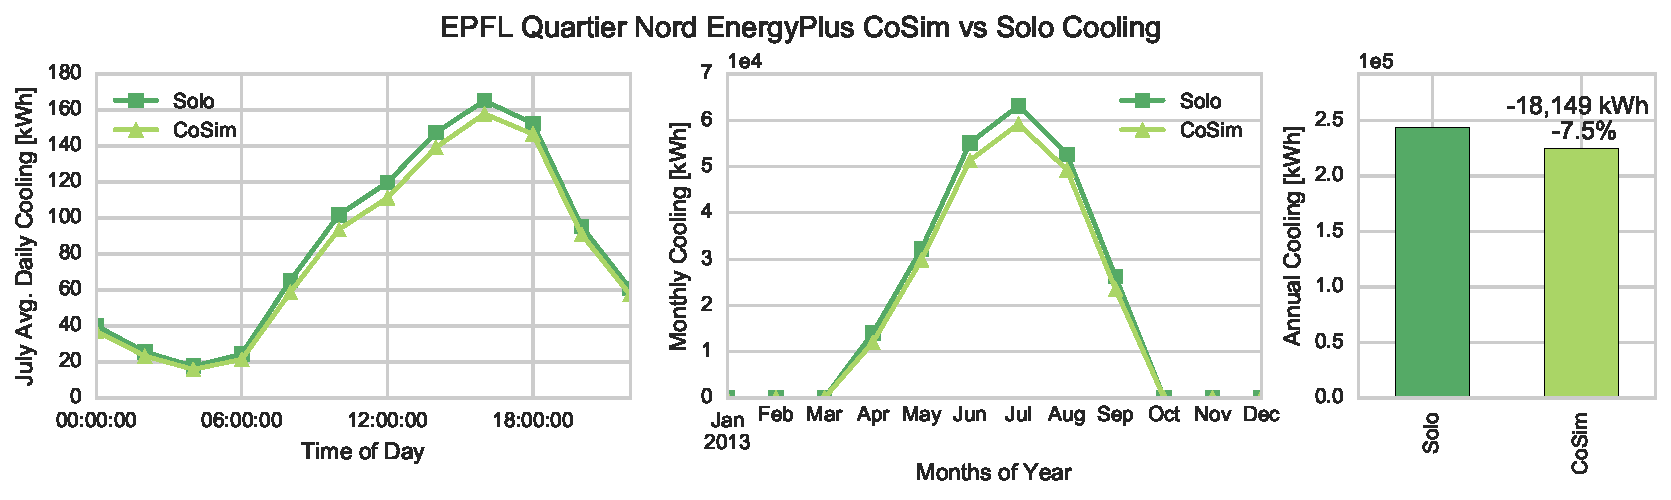
\includegraphics[scale=0.55]{figures/QN_EnergyPlus_Cooling}
\caption{Quartier Nord EnergyPlus Co-Simulation vs. Solo for Cooling}
\label{fig:qn_eplus_cosimvssolo_cooling}
\end{figure}


\begin{figure}[H]
\centering
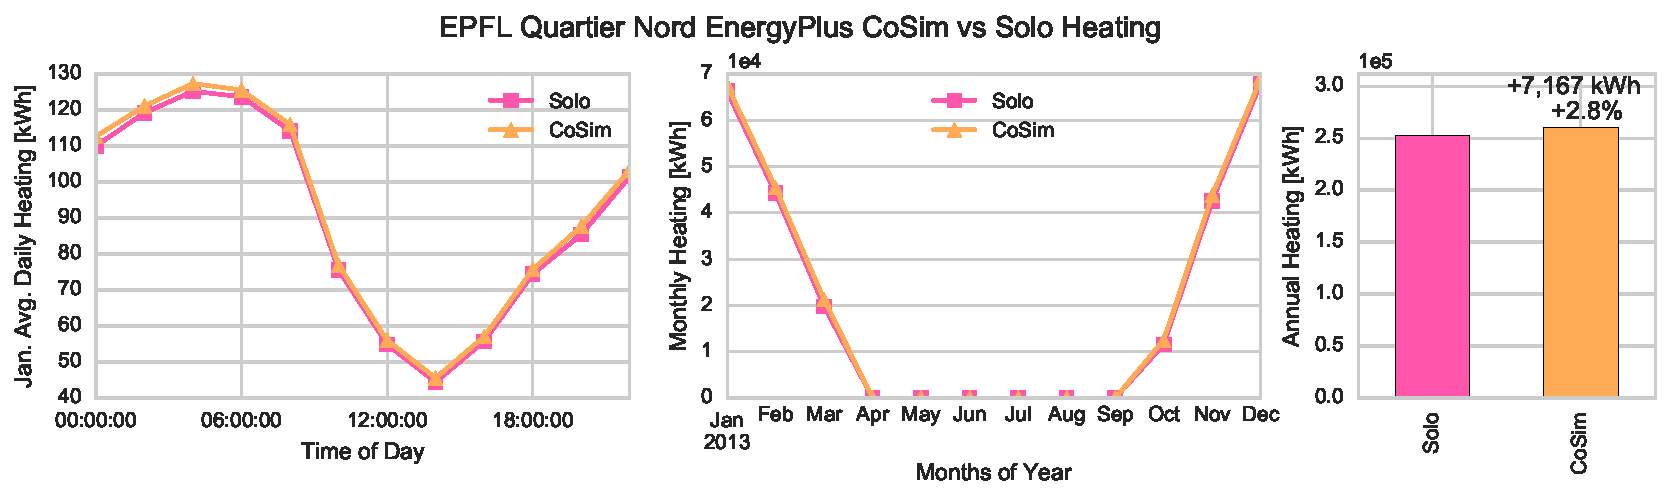
\includegraphics[scale=0.55]{figures/QN_EnergyPlus_Heating}
\caption{Quartier Nord EnergyPlus Co-Simulation vs. Solo for Heating}
\label{fig:qn_eplus_cosimvssolo_heating}
\end{figure}

% \subsection{CitySim co-simulation results}

% When focusing solely on CitySim, a 26.9\% decrease in heating energy is
% observed, as seen in Figure \ref{fig:qn_citysim_cosimvssolo_cooling}. A 49.1\%
% decrease in heating energy is observed, as seen in Figure
% \ref{fig:qn_citysim_cosimvssolo_heating}. These results align with the
% previous comparison of EnergyPlus and CitySim engines. The substantial
% differences between solo and co-simulation in these cases is a result of
% EnergyPlus transferring the heating and cooling load values at each time step. \noteCM{Jerome -- I need some help
% interpreting these results -- you mentioned that there is an expected delta
% between citysim and energyplus in previous studies. Can you help elaborate on
% that?}

% \begin{figure}[H]
% \centering
% 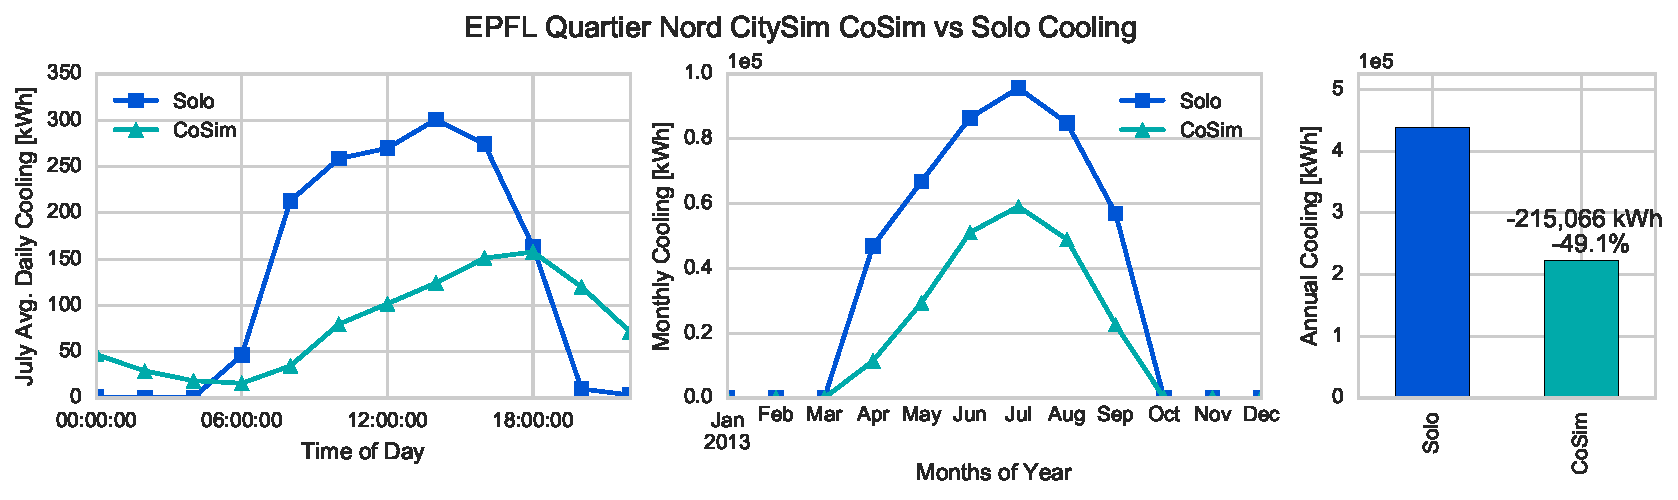
\includegraphics[scale=0.55]{figures/QN_CitySim_Cooling}
% \caption{Quartier Nord CitySim Co-Simulation vs. Solo for Cooling}
% \label{fig:qn_citysim_cosimvssolo_cooling}
% \end{figure}

% \begin{figure}[H]
% \centering
% 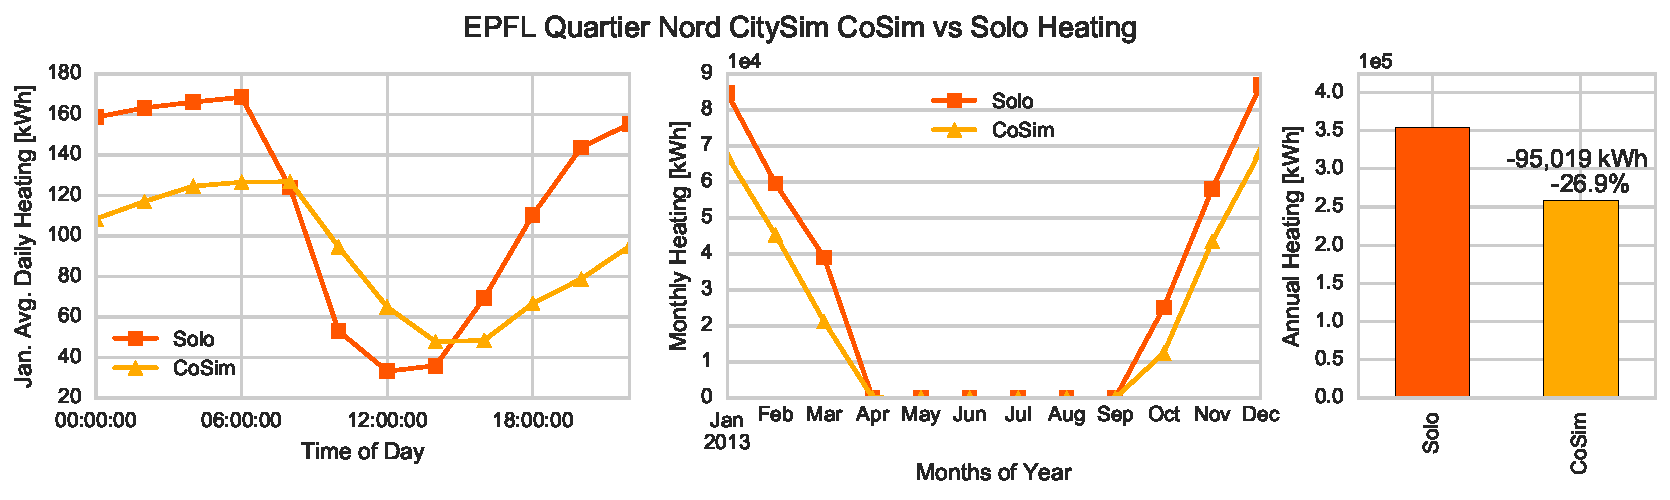
\includegraphics[scale=0.55]{figures/QN_CitySim_Heating}
% \caption{Quartier Nord CitySim Co-Simulation vs. Solo for Heating}
% \label{fig:qn_citysim_cosimvssolo_heating}
% \end{figure}

\section{Discussion}
Two campus case studies were presented in this paper to showcase a novel process of extracting 
model meta-data, conversion of those data into models for two separate simulation engines, and the solo
and co-simulation process of those engines on two real-world case studies. This section will outline 
the advantages and disadvantages of undertaking this process with respect to factors such as 
usability for various applications, simulation speed and resources, and an overview of the tools 
involved in the process.

Advantages of a co-simulation process between EnergyPlus and CitySim were uncovered through
this study. The key advantage is that each of the engines is enabled to account for various 
physical phenomenon in their simulation process that were previously impossible. For example, 
through co-simulation, EnergyPlus was able to utilize the long wave radiation exchange capabilities 
of CitySim. \noteCM{Here we continue the discussion of advantages}

Disadvantages of the co-simulation process are mainly centered upon the increase
in computing time and power needed for the FMI to coordinate data exchange between 
the two simulation engines. \noteCM{Here we continue the discussion of disadvantages}


\section{Conclusion}
The ability to couple and leverage the best aspects of multiple simulation
engines can enhance the modeling of large scale urban agglomerations. This
paper has outlined two such scenarios in which the building-focused EnergyPlus
simulation engine is coupled and co-simulated with the urban-scale CitySim
engine. This process is implemented through a fully automated work flow
process that extracts geometry information at the
urban-scale, creates the necessary input information, executes each engine
with information exchange at each time step of targeted variables, and
accumulates the results of analysis. The process has been implemented on
simplified theoretical scenarios in the past and the key innovation with this
work is in implementation on actual case study campuses and targeted
buildings. The results illustrate that the differences between the co-
simulation and solo environments are within range of previous theoretical
models. The results show that there is a noticeable impact 
More reliable results of the magnitude of differences between the
simulation techniques can be extracted from these real-world scenarios. 

Future work in using co-simulation models for buildings and campuses would
more intensively utilize the model results in a practical implementation of
retrofit scenarios or urban-scale energy systems research.

\subsection{Acknowledgments}
The authors would like to acknowledge the ETH Z\"urich Campus Facilities
Department, the EPFL Real Estate and Infrastructure Department, and Emanuel
Thoma for their assistance in this project. This research was funded by the
Competence Center in Energy and Mobility (CCEM) under the Urban Multi-scale
Energy Modeling (UMEM) project. 
% The authors would also like to acknowledge
 % Emanuel Thoma for his work in developing the geometric models.% %
 % \noteDT{We also
% want to acknowledge Emanuel Thoma for his work on the Hoenggerberg model, no?}

\bibliographystyle{tBPS}
\bibliography{UMEM_CoSim}


\end{document}
